% lucidchart: online chart drawing

\documentclass[letter]{llncs}

\usepackage{amssymb}
\setcounter{tocdepth}{3}
\usepackage[pdftex]{graphicx}
\DeclareGraphicsExtensions{.pdf}
\usepackage{caption}
%\usepackage{subcaption}
\usepackage{float}
\usepackage{url}

\usepackage{llncsdoc}
%\usepackage{makeidx}  % allows for indexgeneration
%\usepackage{mathbbold}
\usepackage{wrapfig}

\usepackage{times}
\usepackage{amsmath, amsfonts}
\usepackage{latexsym, amssymb}
\usepackage{setspace}
\usepackage{longtable}
\usepackage{grffile}
%\usepackage{subfigure}
%\usepackage{algorithm}
%\usepackage{algorithmic}
\usepackage{multirow}
\usepackage{supertabular}
\usepackage{listings}
\usepackage[ruled,vlined,linesnumbered]{algorithm2e}
\usepackage{todonotes}
%\usepackage{color}
%\newcommand{\hilight}[1]{\colorbox{yellow}{#1}}
\usepackage{soul}
\newcommand{\hlc}[2][yellow]{{\sethlcolor{#1}\hl{#2}}}

\urldef{\mailsa}\path|dejun@cs.pdx.edu|
\newcommand{\keywords}[1]{\par\addvspace\baselineskip
\noindent\keywordname\enspace\ignorespaces#1}

\begin{document}

%\tableofcontents

\mainmatter  % start of an individual contribution

% first the title is needed
\title{Managing Traceability Links between Specification and Implementation of Hardware/Software Interfaces}
% a short form should be given in case it is too long for the running head
%\titlerunning{Traceability Links between Specifications and Implementations}
%\authorrunning{Dejun Qian}

\author{Dejun Qian}
\institute{Department of Computer Science  \\
Portland State University \\
Portland, OR 97207 \\
dejun@cs.pdx.edu}

\toctitle{Lecture Notes in Computer Science}
\tocauthor{Authors' Instructions}
\maketitle

%\lstset{frame=trBL,language=C,columns=fullflexible,
%  numbers=left,framexleftmargin=6mm,xleftmargin=7mm,framexrightmargin=5mm,
%  basicstyle=\footnotesize\ttfamily, commentstyle=\rmfamily\itshape}
\lstset{frame=trbl,language=C,columns=fullflexible,
  numbers=left,framexleftmargin=6mm,xleftmargin=7mm,framexrightmargin=5mm,
  basicstyle=\footnotesize\ttfamily, commentstyle=\rmfamily\itshape}

\begin{abstract}
Traceability links between specifications and implementations of hardware/software (HW/SW) interfaces play a crucial role in improving the quality of computer systems.
On one hand, HW/SW interfaces are often quite detailed, on low abstraction levels, 
thus demanding fine-grained traceability links.
On the other hand, HW/SW interface specifications are typically stable while their hardware and software implementations are constantly evolving even after their releases, which requires robust traceability links.
In this paper, we present a framework for managing traceability links between specifications and implementations of HW/SW interfaces. 
This framework supports fine-grained traceability links between basic elements of specifications and constructs of implementation languages.
It also supports automatic migration of links as implementations evolve. 
We have implemented a prototype tool, namely coDoc, in support of this framework. 
We have applied coDoc to ten versions of three virtual devices in the QEMU virtual machine.
Experimental results show that our framework fully supports the types of traceability links between the virtual devices and their specifications,
and it accurately migrates valid links from version to version.
%\keywords{Software Engineering, Data Model}
\end{abstract}



% introduction - give the problem (create and manage links)
% maintenace is important, takes time. 
% reason: code size, spec size, relationship

% the lowest level HW/SW interface primitive is found in the form of SW programmable registers. 
% There are other vital aspects of the HW/SW interface, such as interrupts but these are not covered within the scope of this paper.
% the software interface of an IP block as an address-mapped bus (from processor) being mapped into registers that provide the configuration, control and status interface of the hardware logic.
\section{Introduction}
\label{sec:introduction}

The majority of software engineering work is devoted to maintaining legacy software systems other than developing new ones \cite{abran_maintenance_1991}.
It is estimated that up to 60\% of software maintenance time is spent on program comprehension \cite{lawrence_software_2006}.
Software developers often find it difficult to extract the knowledge about a software system,
because the knowledge is often implicitly expressed,
and distributed in a variety of software artifacts.
Examples of software artifacts include source code, design documents, application programming interface specifications, bug reports, etc.

To make the knowledge about a software system explicit,
reserachers have built various techniques to recover the semantic connections among software artifacts,
especially between documentation and source code \cite{antoniol_recoveringtraceability_2002} \cite{deLucia_incremental_2006} \cite{marcus_recovering_2003}.
These semantic connections are often called \textit{traceability links}. 
Effectively maintaining the traceability links can help improving the productivity of the developer and the quality of the software \cite{neumuller_case_2006}.

Unfortunately, these techniques are not ready to be applied to implementations and specifications of HW/SW interfaces,
even though these implementations are an important category of software that caused most of the system failures in both Windows and Linux operating systems \cite{swift_os_2003} \cite{chou_os_2001},
HW/SW interface forms the interaction point of hardware and software,
and defines the protocol for the hardware and software to communicate.
The implementation of HW/SW interfaces refers to hardware design, device drivers and virtual device prototypes, who implement the communication logic on both sides of the interfaces.
%The implements are designed for a variety of computer components, and form a large part of operating systems and virtual machines.
HW/SW interface specifications describe the HW/SW interfaces in natuaral lagnguage,
and guide the implementation of the interfaces.
HW/SW interface specifications play a crucial role in the comprehension and maintenance of the implementations of the interfaces.
The reason why existing traceability link recovering techniques do not work for HW/SW interfaces is that these traceability links need to be fine-grained,
which is not supported by the existing techniques.
HW/SW interfaces are mainly composed of software-programmable hardware registers mapped to the processor's address space.
The low-level abstraction of the software/hardware interface makes the traceability links fine-grained.
Traceability links between the specifications and implementations usually connect statements, which operate the registers, or expressions, which represent certain bits of registers, to the register bit descriptions in the specifications. 
However, previous tools usually maintain tracebility links between the classes or functions of the source code and sections or paragraphes of the documentation, which is more coarse-grained.

% Second, the evolution nature of software artifacts makes the situation even worse.
% No matter how the traceability links are created -- automatically or manually, these links are probably only valid for a certain version of the software.
% As software evolves during the development and maintenance process, software artifacts changes as well.
% These changes might invalidate the existing traceability links.
% For automatically recovered links, we can re-run the traceability recovery tool to reestablish them.
% However, this solution is computationally costly for interactive use during software development stage.
% For manually recovered links, we must reestablish these links manually again, which is arduous.
% This intimidate people from using these tools in their daily work.

% Second, previous traceability link recovering approaches use information retrieval techniques which have the assumption that all software artifacts are plain texts, and the key words in the texts can express the semantic information of the software artifacts precisely.
% These key words form the digital fingerprint of the software artifacts, and the digital fingerprints for the related software artifacts are highly similar, while the digital fingerprints for unrelated software artifacts are highly different.
% The assumption for IR techniques does not hold for device drivers and device specifications.
% People usually organize device specification by hardware modules and the registers inside the hardware modules.
% The semantic information is often encoded into binary numbers, and presented in tables.
% These modules and registers do not relate to the code in an explicit way.

We present a framework for managing traceability links between specifications and implementations of HW/SW interfaces. 
This framework supports fine-grained links between basic elements of specifications and constructs of implementation languages.
We design a data model to support the framework, and organize the data for the traceability links.
Our framework also supports automatic migration of links as implementations evolve. 

We have implemented a prototype tool, namely coDoc, in support of this framework. 
With this tool, the developer can import and manage implementation source code and interface specifications, select a certain piece of implementation (POI) and a certain piece of specification (POS) of interest, create a traceability link connecting the seleted POI and POS, check out a different version of source code, review and verify the existing traceability links. 
We applied coDoc to three virtual device prototypes and their specifications, recovered traceability links, and verified the traceability links on other versions of the driver code.
Experimental results show that our framework fully supports the types of traceability links between the virtual devices and their specifications,
maintain traceability links with required granularity, 
and it accurately migrates valid links from version to version.
\todo{the data need to be updated}\hlc{It preserves 70\% of the existing traceability links when code evolves to a new version.}

This paper makes the following key contributions:
\begin{itemize}
\item Presented a framework for managing traceability links between specifications and implementations of HW/SW interfaces with accuracy, robustness and fine-granularity.
\item Developed coDoc, a tool implementing the approach.
\item Evaluated our approach with realistic examples.
\end{itemize}

The rest of the paper is organized as follows. 
Section \ref{sec:problem} examplifies and defines the problem that we address in this paper.
Section \ref{sec:approach} and section \ref{sec:implementation} illustrate the design and implementation details of our approach.
Section \ref{sec:evaluation} provides some preliminary evaluation results.
Section \ref{sec:related} reviews the related work.
We conclude our approach and discuss the future work in Section \ref{sec:conclusion}.



% problem and definition - example to illustrate the problem (further illustrate the problem)
% emphasize the special characteristic of hardware-related software
\section{Problem in Managing HW/SW Interface Traceability Links}
\label{sec:problem}

An interface between hardware and software is typically composed of registers exposed by hardware devices and accessible by software. The implementation of the interface should conform to the specification in order to function correctly. Suppose we have to maintain and understand this implementation, we need to establish the relationships between the implementation and the specification.
\begin{figure}[h!]
  \begin{center}
    \begin{tabular}{c}
\begin{minipage}[b]{\linewidth}
  \centering
  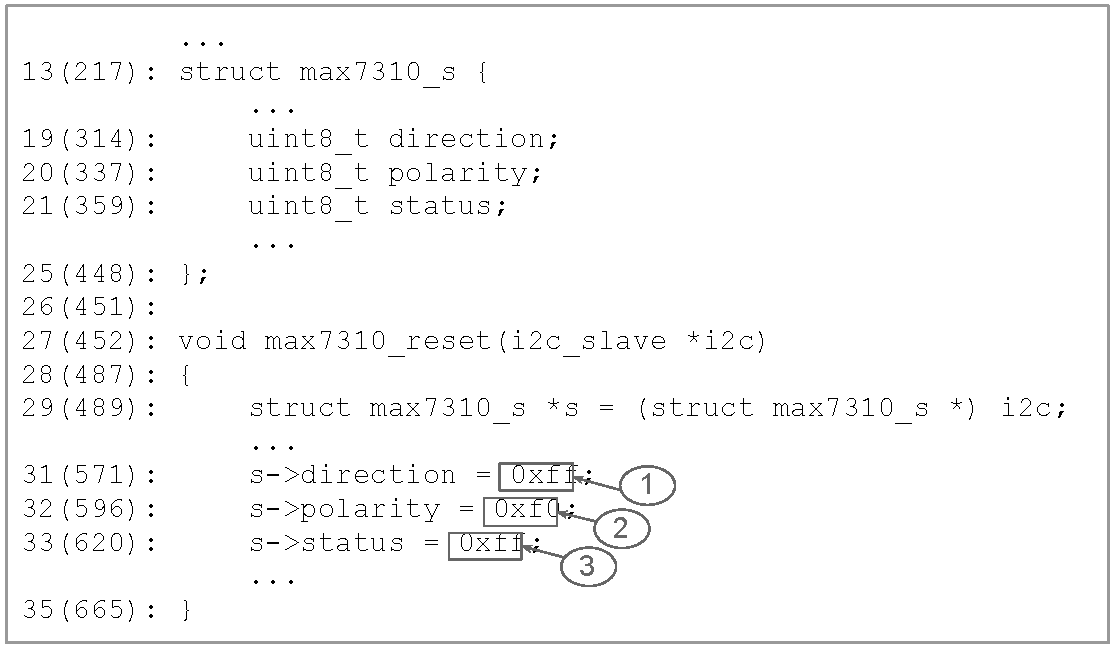
\includegraphics[width=0.8\linewidth]{code1}
\end{minipage}\\
(a) Older Version\\
\\
\begin{minipage}[b]{\linewidth}
  \centering
  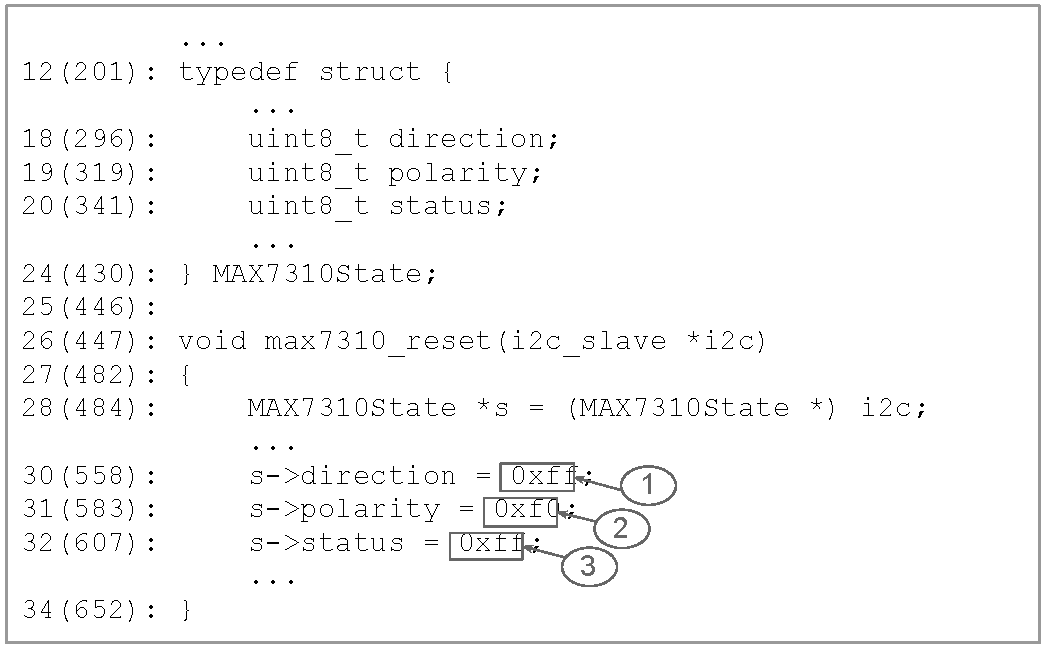
\includegraphics[width=0.8\linewidth]{code2}
\end{minipage}\\
(b) Newer Version
\end{tabular}
  \caption{ Corresponding code snippets from two versions of the MAX7310 virtual device from the QEMU virtual machine. This code defines a function to reset the device.}
  %However, it is unclear why the registers are reset to the values labeled 1, 2 and 3. To know the answer, one has to refer to the specification.}
\label{fig:code}
\end{center}
\end{figure}
Figure~\ref{fig:code}(a) presents part of code extracted from the MAX7310 virtual device from QEMU. A virtual device is a software implementation emulating a hardware device. MAX7310 is a 8-bit I/O port expander. QEMU (Quick EMUlator)~\cite{Bellard05} is a virtual machine widely used in industry to assist hardware-related software development. The source code for this implementation is written in the C language. From the name of the function, we can guess it is trying to reset the device to its initial state. However, we cannot figure out what the values in the right sides of the assignment statements mean only by reading the code here. Figure~\ref{fig:spec} includes the information extracted from the specification of MAX7310. In this figure, we can see three tables for three registers: polarity register, direction register, and status register. These tables present the bit arrangement and the default value for each register. We can see that the values used in the code are defined in the specification. The code uses the hex format, and the specification uses the binary format. The piece of code and the piece of specification labeled with the same number are related, which means the piece of specification explains the piece of code with the same label.

\begin{figure}
  \centering
  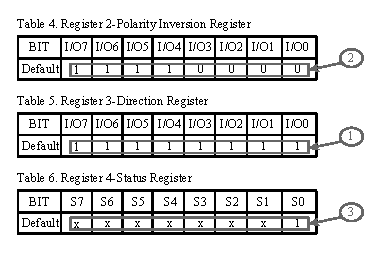
\includegraphics[width=0.7\textwidth]{spec}
  \caption{Specification Example. This is part of the MAX7310 specification, including three tables which define default values for three registers.}
  \label{fig:spec}
\end{figure}

% in the directory including max7310.c: git log --follow --all -p max7310.c > a.txt
Implementation code evolves all the time in its lifecycle. By checking the QEMU repository, we found that the first version of the code in Figure~\ref{fig:code} was created on May 23, 2007, and the last change was on May 1, 2013. This code has changed 21 times till now, and it still keeps changing.
Figure~\ref{fig:code}(b) shows a newer version of the code in Figure~\ref{fig:code}(a). Line 13, 25 and 29 of the code in Figure~\ref{fig:code}(a) has changed to the line 12, 24 and 28 in Figure~\ref{fig:code}(b). Compared to code, specification is often relatively stable. The specification in Figure~\ref{fig:spec} only has three versions, and the last change happened in 2005. The specification remains unchanged since the code was created.

This example, although simple, reveals three basic requirements for managing traceability links between specification and implementations as follows.

\smallskip
\noindent 
\textbf{Requirement 1:} Traceability links should be able to uniquely identify and accurately locate relevant pieces of code in the source file and pieces of specification in the specification file. As in the example, there should be a simple and unique way to locate the code pieces and specification pieces surrounded by the boxes labeled by 1, 2 and 3.

\smallskip
\noindent
\textbf{Requirement 2:} Traceability links should be able to provide references on the statement level or expression level for source code and at the sentence level or word level for specification. As in this example, the code pieces and specification pieces surrounded by the boxes labeled by 1, 2 and 3 are all on the expression level and the word level.

\smallskip
\noindent
\textbf{Requirement 3:} Traceability links should be immune from the evolution of unrelated code. We need to ensure that an identifier created for the old version of code works for the new version if the code piece referred to by the identifier does not change.



% the design and data model (a general framework to solve the problem) - key as a requirement
\section{Our Approach}
\label{sec:approach}

We first present an overview of our approach. Then, we propose the underlying data model. The data model introduces the requirement \hlc{of the} techniques to represent the POIs and the POSes. We illustrate how our approach address this problem at last.

\subsection{Overview}
\todo{this section need rewriting. focus on data.}
\begin{figure}
\begin{center}
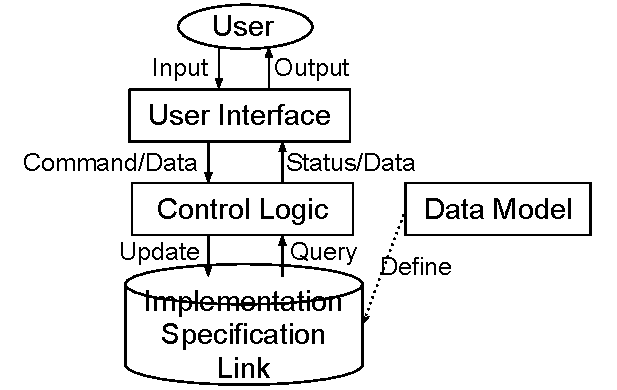
\includegraphics[width=0.55\textwidth]{framework}
\caption{Framework of Our Approach.}
\label{fig:framework}
\end{center}
\end{figure}

As shown in Fig.~\ref{fig:framework}, the framework of our approach consists three components: database, control logic, and user interface. The structure of the traceability link data in the database is defined by the data model. Control logic lays in the middle of user interface and datamodel. It receives and processes command from the user interface. Depending on the command, it either updates the database, or queries the data in the database and report the result to the user interface. User interface is responsible of communicating with the end user, processs and passes the input from user to the control logic, get the result from the control logic and present the result to the user.



\begin{figure}
\begin{center}
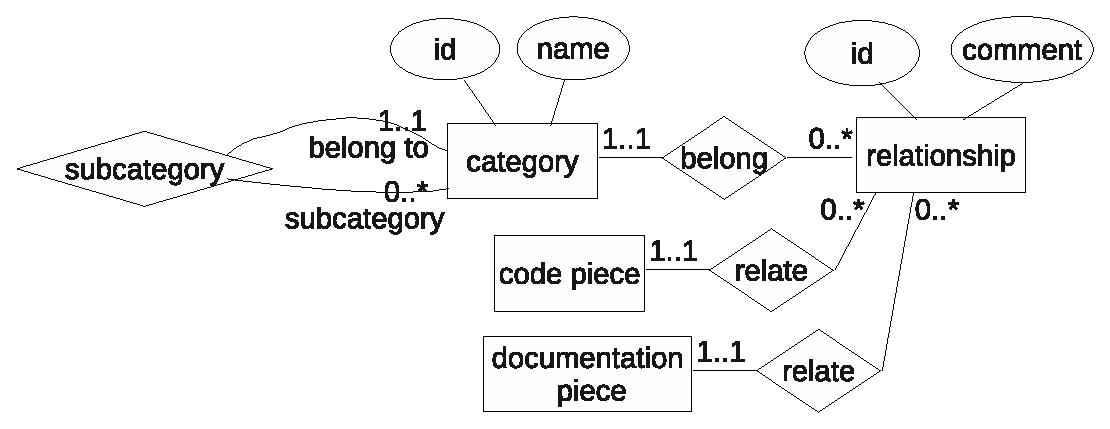
\includegraphics[width=0.85\textwidth]{datamodel}
\caption{Data Model. Entity-Relation Model is used. Rectangles represent entity sets. Ovals represent attributes. Diamonds represent relationships.}
\label{fig:datamodel}
\end{center}
\end{figure}

\subsection{Data Model}
The data model is the key to support fine-grained links between basic elements of specifications and semantic constructs of implementation languages and automatic migration of links as implementations evolve. We introduce the data model of our approach in this section.

The data model describes the data objects being handled in the framework, their attributes, and the relationships between these data objects.
Fig.~\ref{fig:datamodel} presents the data model of our design.
Entiry-relationship model is used.
Rectangles represent entiry sets.
Ovals represent attributes.
Diamonds represent relationships.
We have four entity sets in our design: code file mark, spec file mark, code piece anchor and specification piece anchor.
Code piece anchor and specification piece anchor represent the selected code and specification piece respectively.
Both code file mark and spec file mark entities have attributes id and path:
id is a 128-bit number, and serves as the key of the entity;
path is the file path pointing to a file in the local machine. % not a key, it may change
Code piece anchor and spec piece anchor have id and path as attributes:
id is a 128-bit number, and serves as the key;
path points to the code or spec piece.
Traceability links are represented by the relationships between code piece anchor and spec piece anchor.

Special attention should be paid to four attributes: path for code file, path for spec file, path for code piece anchor and path for spec piece anchor.
\todo{explain}\hlc{These four attributes are foreign keys used to refer to data that do not exist in database.}
As foreign keys, these attributes should be able to uniquely identify the entities they refer to.
The path provided by the file system is a solution to the path for code files and spec files, as we can easily identify both code files and spec files by these pathes.
The pathes for anchors are challenging, little work has been done to address this problem.

%Based on the model above, we can conclude the schema as following.
%Examples?

\subsection{Anchor Design}

Anchors includes specification anchor and implementation anchor. The three basic requirements for traceability links are the constraints for the design. We present how our approach make these requirements fulfilled. Specification anchor design is addressed first, then we present the implementation anchor design.

\subsubsection{Spec Anchor}

Specifications are relatively stable, which make the specification anchor design easier than implementation anchor. Using the absolute coordinate is enough to meet the requirements. Most of the HW/SW interface specification are in PDF format. We use this format to present our approach. Basically, the coordinate for specification piece is denoted by two points -- the point representing the beginnings of the selection and the point representing the end of the selection. Each point is denoted by a vector $<$page, x-coord, y-coord$>$, where page is the page number the point located, x-coord and y-coord are the horizontal and vertical coordinate respectively.

The method is accurate as each point is uniquely represented by the coordinate. This method is also fine-grained, because this method could represent each word, sentence or evan arbitrary size of POS. The method is not robust as it uses the absolute coordinate as the basic element of the anchor. However, specifications are relatively stable, which makes this approach work most of the time.


\subsubsection{Offset-Based Anchor}

Similar to specification anchor,
absolute coordinates also fit the situation of implementation anchor.
Basically, implementation code is just a string of ASCII charactors. 
Each piece of code is a substring of this string.
We can use the offset of the substring in the string and the length of the piece of code to represent this piece of code.
The pair (offset, length) is called Offset-Based Anchor.
Fig.~\ref{fig:code}(a) illustrate this technique.
The parenthesized number in front of each line represent the offset of the first charactor of that line.
Using this approach, we can get the Offset-Based Anchors for the three code pieces labeled 1, 2 and 3 as (590, 4), (614, 4) and (635, 4) respectively.

The advantage of this technique is obvious, it is simple and provides fine-grained traceability. The disadvantage of this technique is that these anchors fail after the code evolves. Fig.~\ref{fig:code}(b) is the code after the code in Fig.~\ref{fig:code}(a) evolves. We can see the anchors we get above do not point to the previous pieces of code anymore. The reason is that this approach is context sensitive. By saying context sensitive, we mean it depends on its context. In this approach, the anchor depends on the number of charactors preceeding the piece of code.

One way to overcome this disadvantage is to get the knowledge of change to keep the links valid. However, this information is not always available. Most of the time, code is changed by other people. We can only get the changed result without how the change is made.

% a figure example
\begin{figure}[h!]
  \begin{center}
    \begin{tabular}{c}
\begin{minipage}[b]{\linewidth}
  \centering
  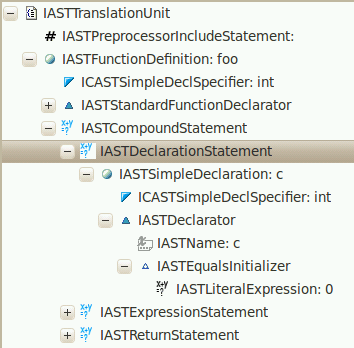
\includegraphics[width=0.8\linewidth]{ast1}
\end{minipage}\\
(a) AST for the Code in Fig.~\ref{fig:code}(a)\\
\\
\begin{minipage}[b]{\linewidth}
  \centering
  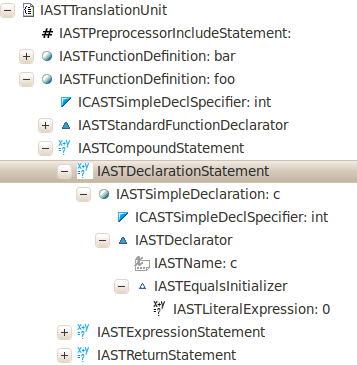
\includegraphics[width=0.8\linewidth]{ast2}
\end{minipage}\\
(b) AST for the Code in Fig.~\ref{fig:code}(b)\\
\\
\begin{minipage}[b]{\linewidth}
  \centering
  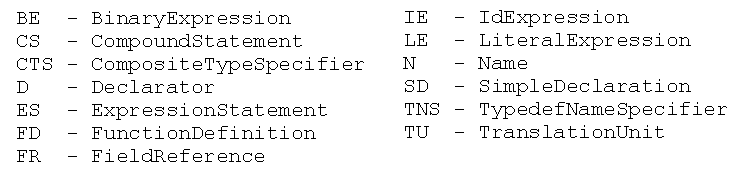
\includegraphics[width=0.95\linewidth]{ast_legend}
\end{minipage}
\end{tabular}
\caption{The AST for the implementation code in Fig.~\ref{fig:code}.}
\label{fig:ast}
\end{center}
\end{figure}

% syntax tree, a string of syntax tree leaf nodes.
% content-free (make immune from change of the content) vs content-sensitive (make unique)
% evaluate on unique
\subsubsection{Syntax Tree Based Anchor}
To make the traceability links created for one version of code work for other versions,
we need a robust strategy to represent the code pieces.
More specifically, we need to find some properties of the code that are relatively stable when code evolves.
These properties can serve as keys to identify the code piece.
We use syntax information to form the main element of our code piece identifier.
The code can be parsed and represented by a parse tree or an abstract syntax tree (AST).
We use AST in our approach, as it faithfully retains the structure of the original source code, and is concise and efficient to compute compared to parse tree.
AST usually has fewer nodes than parse tree, and takes less time to traverse.
Each node in AST tree represents a syntax unit of the grammer,
a parent of a node represent a bigger grammer unit that includes the grammer unit represented by the child node.
The nodes are labeled by the type of the grammer unit.
For each leaf node, we also include the value, which is the code this node represents, in the label.
For some of the inner nodes that have a name, we also include the name in their labels. For example, a inner node that represents a function will be labeled with the grammer unit type and the name of the function.
A change of the code in one branch of AST usually does not affect the structure in other branches.
Representing code pieces based on the structure in the syntax tree is robust.
Fig.~\ref{fig:ast}(a) and Fig.~\ref{fig:ast}(b) are the Abstract Syntax Trees (AST) for the code in Fig.~\ref{fig:code}(a) and Fig.~\ref{fig:code}(b).
Dot lines represent branches not shown.
Fig.~\ref{fig:ast}(a) shows two subtrees of the root.
The left subtree represents line 13 - line 25 of Fig.~\ref{fig:code}(a), which defines the structure max7310\_s.
The right subtree represent line 27 - line 35 of Fig.~\ref{fig:code}(a), which defines the function max7310\_reset.
Similarly, the left subtree of the AST in Fig.~\ref{fig:ast}(b) represent line 12 - line 24 in Fig.~\ref{fig:code}(b), and the right subtree represents line 26 - line 34.
From the AST shown in Fig.~\ref{fig:ast}(a) and fig.~\ref{fig:ast}(b), we can see that the left tree has changed as the code for structure definition changed.
However, the structure of the right subtree remain the same, unaffected by the change of the left subtree.

Based on the AST of the code, we define our identifier to a piece of code as a sequence of leaf nodes in the AST. Each leaf node is represented by the path from the leaf node to the root of the AST. For example, line 31 in Fig.~\ref{fig:code}(a) is represented by the highlighted three leaf nodes in Fig.~\ref{fig:ast}(a). The leaf nodes are in the same order as they are visited by depth-first search of the AST. For this example, the closest common parent node for these three leaf nodes also represents the same piece of code, and thes representation is even simpler. We avoid using this representation for two reasons: First, this representation contains less information; Second, this representation is sensitive to formatting and style convention. For example, some programmer may prefer no spaces adjacent to the equal sign, or they may insert some spaces besides the equal sign to make it aligned with other lines of assignment statements. Either case will change the string represented by this common parent, and make the traceability link invalid. We will address how we determine if a traceability link is valid or not in the next section.

Using this approach, let's consider the pieces of code label by 1, 2 and 3 in fig.~\ref{fig:code} again. The identifier for these code pieces in AST are shown in fig.~\ref{fig:ast} labeled with the same number.
Through the two ASTs are different, 
the highlighted nodes can be represented by the same path from the roots of these two ASTs.
As a result, we can use this method to identify the piece of code, and the change of the unrelated code does not invalidate the identifier.

This method is relatively stable.
However, it may not uniquely identify a piece of code,
which means one identifier may refer to two or more pieces of code.
The pieces of code label by 1 and 3 in fig.~\ref{fig:ast}(a) showes two pathes that are encoded as the same identifier -- $<$\texttt{LE:0xff/BE/ES/CS/FD:max7310\_reset/TU}$>$.
As a result, this identifier can not distinguish these two pieces of code, 
and can not serve as a key to these pieces of code.

\subsubsection{Hybrid Anchor}

Offset-based anchor can uniquely identify a piece of code, but it is not immune to code evolusion.
Syntax tree based anchor is immune to code evolusion, but it can not uniquely identify some pieces of code.
We combine these two methods and form hybrid anchor.
For each leaf node that has an ambiguous path representation,
we can always find at least one of its ancesters that has an unique path.
In the worst case, we will get to the root node.
Our approach is composed of two steps.
First, we compute the syntax tree based anchor,
then, we go over the path from leaf to root, find the first node that is a unique identifier.
Second, we compute offset based anchor based on this unique identifier instead of the begining of the whole implementation code.
Consider the AST in fig.~\ref{fig:ast}(a), to identify the piece of code labeled by 1,
we go through the path towards the root,
and get to the first unique identifier at the inner node CS.
The node CS represent line 28 - line 35 of the code in fig.~\ref{fig:code}(a).
It is the body of the function \texttt{max7310\_reset}, and there is only one body for this function by the C language grammer.
The offset based identifier based on this node is (103,4), as the first charactor of the node CS is located at offset 487 and the offset based anchor is (590,4).
We combine the information of the inner node CS and the calculated coordinate to represent the piece of code with no ambiguity.
Same as offset based anchor, if the code does not change, it can uniquely identify the piece of code.
If the code changes, this method still works if the code for the unique identifier remain the same.
Actually, this is a general approach for the previous two.
If we get to the root node while finding the first unique ancestor, then this approach will become the same as offset based anchor.
However, if the lead node itself is the firtst node with unique identifier, then this approach is the same as syntax based anchor.
The lower the node with the unique identifier in AST, the better our approach works.
%However, this method provide redundent information, which can be used to check the validity.

% example?


% handle some specific difficulties - our solution using ast tree
\section{Implementation}
\label{sec:implementation}

This section first presents the architecture of the coDoc prototype tool, which implements our traceability link management framework. After that, we introduce the algorithms for validating the traceability links and for code selection completion which helps users to complete code piece selection when part of a syntax element is selected.

\subsection{Architecture}

The architecture of our approach is shown in Figure \ref{fig:architecture}.
There are three types of data here, 1) code, 2) spec, and 3) traceability links.
These data are consumed by three components: code manager (CM), spec manager (SM) and link manager (LM).
\begin{figure}
\begin{center}
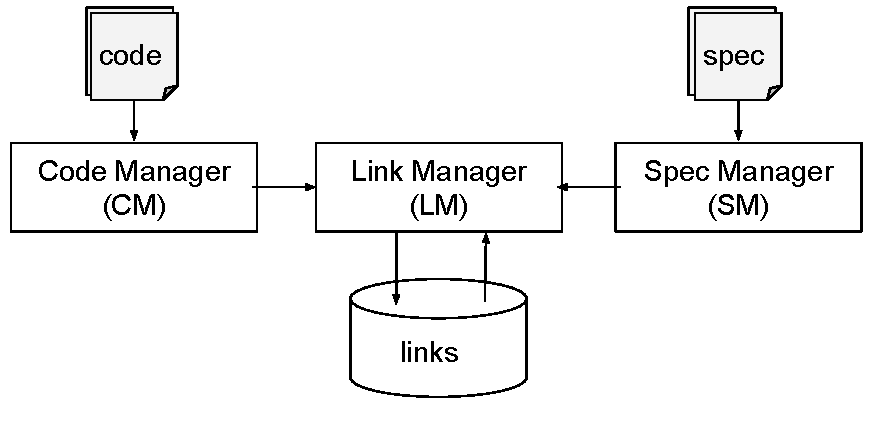
\includegraphics[width=0.55\textwidth]{architecture}
\caption{coDoc Architecture and Features}
\label{fig:architecture}
\end{center}
\end{figure}
\begin{enumerate}
\item \textit{Link Manager.} Traceability link manager gets the highlighted code piece from code manager and the highlighted spec piece from spec manager, and creates traceability link for these two piece of information. It also reads the traceability link data, verifies the validity of the link,
and highlights the code and document pieces that are related.
\item \textit{Code Manager.} Code manager reuses C/C++ Development Tool (CDT) editor from Eclipse~\cite{Eclipse} to parses the code,
and highlights syntax elements. It can highlight the piece of code based on the information provided by the user or the link manager.
\item \textit{Spec Manager.} Spec manager renders the pdf content, can support select and highlight spec content, and communicate with the link manager.
\end{enumerate}

We implemented coDoc as an Elipse Rich Client Program (RCP),
which can make our tool share the appearance in Eclipse that is familiar by many programmer.
Figure \ref{fig:platformview} is the screenshot of the tool.
The bottom is the UI for link manager, while the top middle part and top right side are the UI for code manager and spec manager respectively.
To traverse a traceability link, users can select a link from the list in the link manager or click on a code construct in the code manager. 
As a result, the link, the relevant code, and the relevant spec piece are highlighted in the link, code, and the spec mangers. 

% convert platformview.png platformview.eps
\begin{figure}
\begin{center}
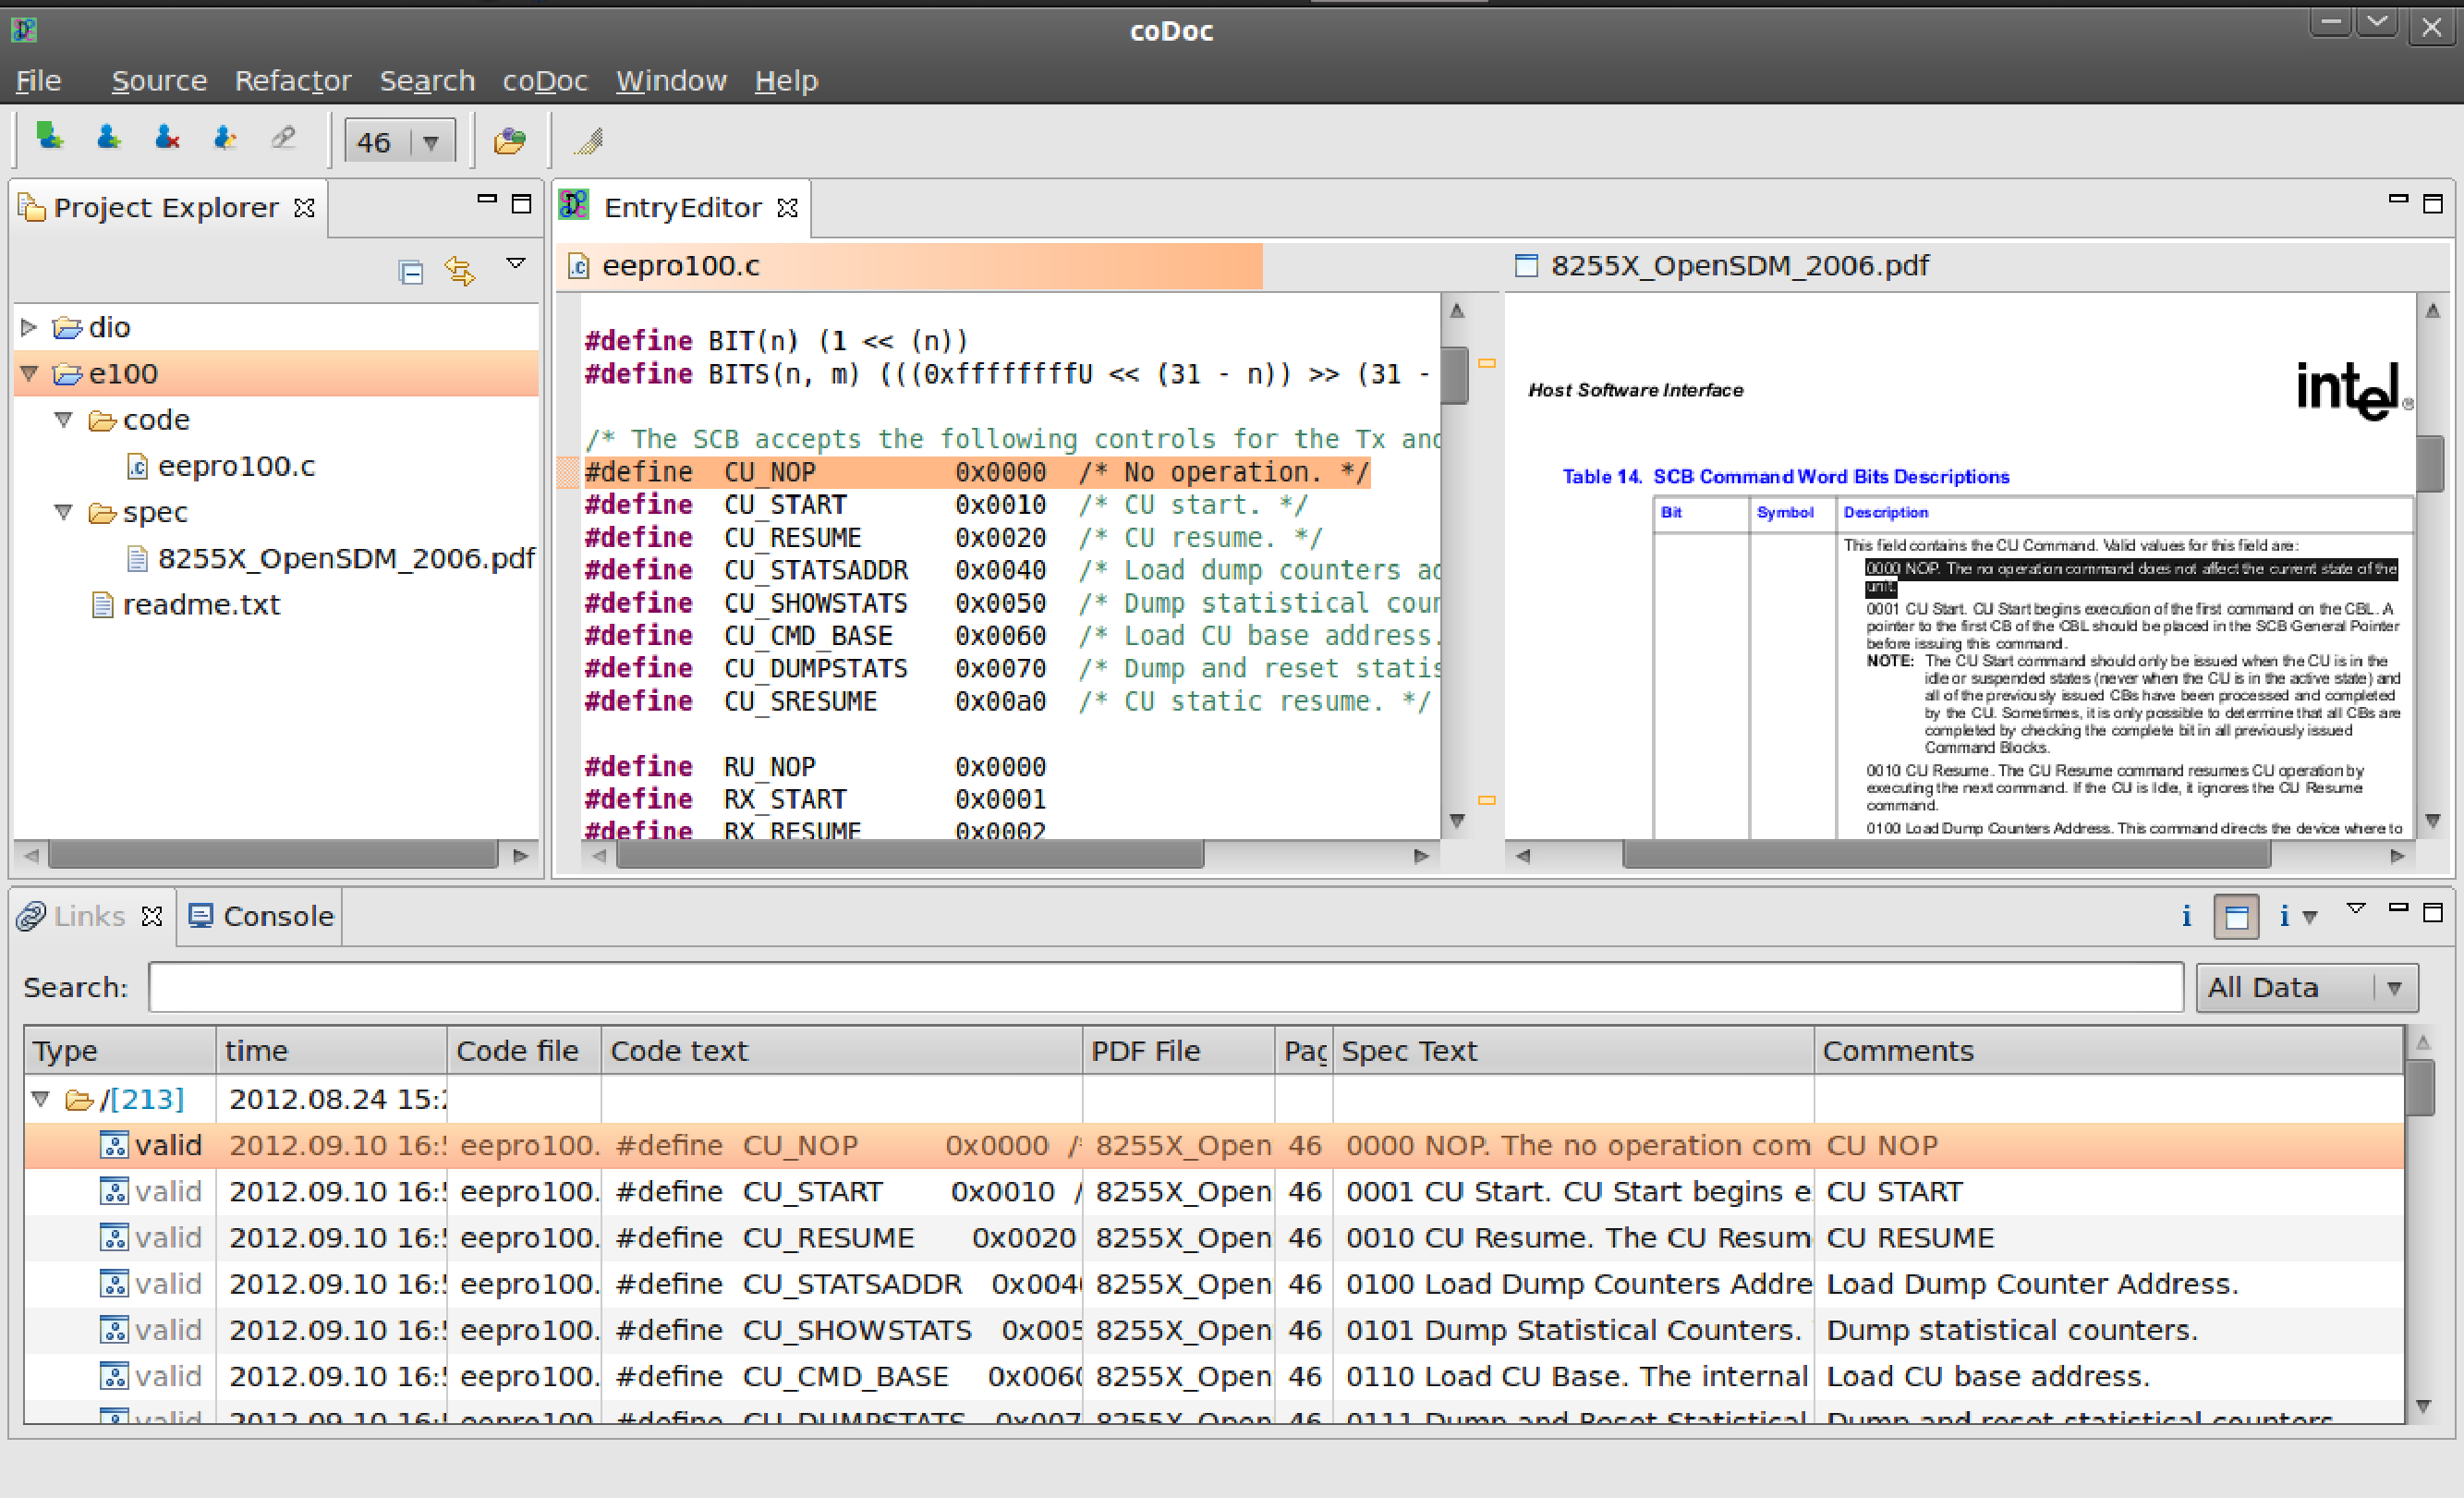
\includegraphics[width=\textwidth]{platformview}
\caption{coDoc User Interface Screenshot}
\label{fig:platformview}
\end{center}
\end{figure}


\subsection{Link Validation}

%\begin{figure}[h!]
%  \begin{center}
%    \begin{minipage}[b]{0.6\linewidth}
%      \centering
%      \renewcommand{\ttdefault}{pcr}
%      \begin{lstlisting}
%for each leaf node in syntax tree
%  for each node in anchor
%    node string compare
%\end{lstlisting}
%\end{minipage}
%\caption{Pseudocode for Link Validation}
%\label{fig:validate}
%\end{center}
%\end{figure}

When code evolves, we need to validate the existing traceability links.
Once an invalid traceability link is found, we report it and ask the user to correct it manually.
To check the validity of the traceability links, we record the content of the code piece and the spec piece when generating the links.
The content is used later to compare with the content to which the path points to when code changes.
The validation process basically goes through each traceability link in the database,
and checks whether the link is valid or not.
\begin{algorithm}[!h]
\DontPrintSemicolon
\SetKwComment{tcp}{\hfill$\triangleright$ }{}
\SetCommentSty{emph}
$AST \leftarrow \textsc{Gen-AST}(code)$\;
$\langle RES, CONTENT_C \rangle \leftarrow \textsc{Get-Code-Content}(AST, link.code.path)$\;
\If{$RES = FALSE$} {
\Return $FAILURE$\;
}
$RES \leftarrow \textsc{Compare-Content}(CONTENT_C, link.code.content)$\;
\If{$RES = FAIL$} {
\Return $FAILURE$\;
}
$CONTENT_S \leftarrow \textsc{Get-Spec-Content}(spec, link.spec.path)$\;
$RES \leftarrow \textsc{Compare-Content}(CONTENT_S, link.spec.content)$\;
\If{$RES = FAIL$} {
\Return $FAILURE$\;
}
\Return $SUCCESS$\;
\caption{$\textsc{Traceability-Link-Validation}(link)$}
\label{alg:validate}
\end{algorithm}
Algorithm~\ref{alg:validate} presents the pseudo-code for check the validation of one single traceability link.
Line 1 - line 7 check the validity of the code piece part of the traceability link.
Line 1 generates the AST for the current code first.
Line 2 then invokes the function \textsc{Get-Code-Content} with the path of the code piece as input, identify the code piece in the new AST, and return the content of the code piece if the code piece is identified successfully.
If the path of the code piece cannot identify any code piece or can identify more than one code piece, the function \textsc{Get-Code-Content} reports failure.
Line 5 compares the the content extracted from the new code with the recorded content, and reports failure if they do not match.
After finishing checking the code piece, line 8 - line 11 of the algorithm check the spec piece in a similar flow.
If no failure happens, the algorithm returns successfully at line 12.


\subsection{Code Selection Completion}

%To improve the user experience of coDoc, we help users to select the code pieces when creating traceability links.
The coDoc tool assists user to select the code pieces that can be used in traceability links. Each code piece selected is required to be a complete language construct.
%Our approach is based on the fact that it is usually meaningless to have part of the basic code elements as the code piece of the traceability links.
For example, we do not create a link between part of a variable name in the code and part of a word in the spec.
We assume that every selected piece of code is composed of valid syntax elements.
Based on this assumption, we can help users to automatically complete their selection when they only select part of a syntax element such as a variable. 
Algorithm \ref{alg:completion} outlines our approach.
\begin{algorithm}[!h]
\DontPrintSemicolon
\SetKwComment{tcp}{\hfill$\triangleright$ }{}
\SetCommentSty{emph}
$AST \leftarrow \textsc{Gen-AST}(code)$\;
$LEAF\_SEQ \leftarrow \textsc{Gen-Leaf-Sequence}(AST)$\;
$AST\_selection \leftarrow \textsc{To-AST-Based}(LEAF\_SEQ, original\_offset)$\;
$new\_offset \leftarrow \textsc{To-Offset-Based}(AST\_selection)$\;
\Return $new\_offset$\;
\caption{$\textsc{Complete-Code-Selection}(orginal\_offset)$}
\label{alg:completion}
\end{algorithm}
This algorithm takes a code selection in the offset based format,
and returns a new, appropriately enlarged code selection in the offset based format.
We choose offset based format because Eclipse use this format to highlight code pieces.
The algorithm basically works as follows: (1) lines 1 - 3 align the input offset-based selection to its smallest enclosing language construct by analyzing the AST.
(2) line 4 maps the enlarged code selection to the offset based format and returns it.  
As we discussed above, the AST based selection is a sequence of AST leaf nodes in the depth-first-search order, which is the same order as the code in the source code.
The AST based code piece covers all the meaningful part of the original offset based code piece.
To transform the offset based selection to the AST based selection,
we obtain the sequence of leaf nodes of the AST in line 1 and line 2,
and then match the leaf node sequence with the offset-based selection to get the enlarged AST based selection.
The leaf nodes in the AST based selection is determined as follows: if a leaf node contains any part of the offset selected code, then the leaf node is in the AST based selection.
After we obtain the AST based selection, we transform it back to a new, enlarged offset based selection, and display it to users.
Each time users make a selection, coDoc adjusts the selection to valid syntax boundary.



%evaluation - three vd with ten version
\section{Evaluation}
\label{sec:evaluation}

\subsection{Experimental Setup}
\todo{The data in the section are fake.}
We evaluate our approach on four virtual device prototypes in QEMU. QEMU is a generic and open source machine emulator, which can host unmodified guest operating systems \cite{bellard_qemuwiki_2013} \cite{bellard_qemu_2005}. QEMU includes virtual implementations for a large number of hardware devices. We do our evaluation on four of them: MAX7310, RTL8139, EEPro100 and E1000. MAX7310 is a 8-bit I/O expander developed by Maxim. This device is used when a system need more I/O ports. EEPro100, E1000 and RTL8139 are three popular network adapters. Both EEPro100 and E1000 are developed by Intel, and RTL8139 is developed by Realtek. All these four devices have specifications in PDF (Portable Document Format) format. We examined the release history of the virtual implementations and specifications of these four hardware device, and found that almost no change has been made to specifications after the corresponding implementations have begun to release.

Based on the QEMU repository, the virtual device prototypes for MAX7310, RTL8139, EEPro100 and E1000 have 22, 143, 163 and 168 versions since they are first created. We check out ten stable versions of all these virtual device drivers from the repository. 
The ten versions we used are stable-0.10, stable-0.11, stable-0.12, stable-0.13, stable-0.14, stable-0.15, stable-1.0, stable-1.1, stable-1.2 and stable-1.3, we represent them as 1 - 10 repectively.
We present the average lines of code (LOC) and the average number of functions of the virtual device prototypes, as well as the number of pages of the specifications in Table \ref{table:vdd}.
The LOC metrics are measured by the tool named locmetrics.
The lines of code (LOC) range from 181 to 2771. The sizes of specification range from 15 pages to 410 pages.

The changes from version to version for all the four virtual device prototypes are shown in Table \ref{table:version}. The changes are measured by the lines of code different from version to version using an open source tool cloc.

\begin{table}[th]
\caption{Three Virtual Device Drivers Used for Evaluation}
\centering
\begin{tabular*}{0.6\textwidth}{@{\extracolsep{\fill}}rccc}
\hline
 & \multicolumn{2}{c}{implementation} & specification \\
\cline{2-4}
 & LOC & Functions & pages \\
\hline
MAX7310 & 181 & 9 & 15\\
RTL8139  & 2771 & 101 & 67\\
EEPro100  & 1870 & 64 & 175\\
E1000  & 1905 & 52 & 410\\
\hline
\end{tabular*}
\label{table:vdd}
\end{table}


\begin{table}[th]
\caption{The Changes in Ten Versions}
\centering
\begin{tabular*}{0.9\textwidth}{@{\extracolsep{\fill}}rccccccccc}
\hline
 & 1-2 & 2-3 & 3-4 & 4-5 & 5-6 & 6-7 & 7-8 & 8-9 & 9-10 \\
\hline
MAX7310 & 32 & 28 & 0 & 0 & 18 & 0 & 24 & 0 & 0\\
RTL8139 & 50 & 349 & 120 & 41 & 432 & 116 & 123 & 9 & 88\\
EEPro100 & 81 & 765 & 903 & 22 & 304 & 231 & 135 & 21 & 2\\
E1000 & 64 & 199 & 39 & 42 & 80 & 120 & 198 & 25 & 27\\
\hline
\end{tabular*}
\label{table:version}
\end{table}

% accuracy
\subsection{Accuracy}
We measure the accurary by the number of uniquely identifiable POC over number of traceability links recovered for all the virtual prototypes. The result is shown in Table \ref{table:accuracy}

\begin{table}[th]
\caption{Accuracy}
\centering
\begin{tabular*}{0.3\textwidth}{@{\extracolsep{\fill}}rc}
\hline
 & accuracy \\
\hline
MAX7310 & 80\%\\
RTL8139  & 87\%\\
EEPro100  & 78\%\\
E1000  & 91\%\\
\hline
\end{tabular*}
\label{table:accuracy}
\end{table}

% granularity
\subsection{Granularity}

The identifying method with fine granularity makes the relationship created by coDoc very accurate, 
80\% of the code pieces are marked inside the statement and expressions.
The same result happens for the document.
In the whole relationships, 
90\% of the document pieces are marked on cells in the tables.
The granulariy results are listed in Table \ref{table:granularity}.

\begin{table}[th]
\caption{Granularity Result}
\centering
\begin{tabular*}{0.6\textwidth}{@{\extracolsep{\fill}}rccc}
\hline
 & \# functions & statements & expressions \\
\hline
MAX7310 & 108 & 2 & 3\\
RTL8139  & 213 & 4 & 5\\
EEPro100  & 213 & 4 & 5\\
E1000  & 213 & 4 & 5\\
\hline
\end{tabular*}
\label{table:granularity}
\end{table}

%In our own experience, we found that the ability to see the code, 
%the documentation and the relationships on the same screen saves a lot of time,
%as we don't need to switch between different tools.

\subsection{Adapting to Evolving Code}

To evaluate how our approach adapt to evolving code, we recover the traceability links for the first version of all the four virtual device driver code.
We then check the number of valid traceability links left in the later versions. The result is shown in table \ref{table:robust}.
% traceability link lifetiem (versions)

\begin{table}[th]
\caption{Robustness}
\centering
\begin{tabular*}{0.9\textwidth}{@{\extracolsep{\fill}}rccccccccc}
\hline
 & 1-2 & 2-3 & 3-4 & 4-5 & 5-6 & 6-7 & 7-8 & 8-9 & 9-10 \\
\hline
MAX7310 & 108 & 2 & 10 & 108 & 2 & 10 & 108 & 2 & 10\\
RTL8139  & 213 & 4 & 210 & 108 & 2 & 10 & 108 & 2 & 10\\
EEPro100  & 213 & 4 & 20 & 108 & 2 & 10 & 108 & 2 & 10\\
E1000  & 213 & 4 & 290 & 108 & 2 & 10 & 108 & 2 & 10\\
\hline
\end{tabular*}
\label{table:robust}
\end{table}

\subsection{Performance}

We test the performance of our algorithm to complete code selection and to verify traceability links. The result is shown in table \ref{table:performance}.

\begin{table}[th]
\caption{Performance}
\centering
\begin{tabular*}{0.6\textwidth}{@{\extracolsep{\fill}}rccc}
\hline
 & verification & completion\\
\hline
MAX7310 & 108 & 2 \\
RTL8139  & 213 & 4\\
EEPro100  & 213 & 4\\
E1000  & 213 & 4\\
\hline
\end{tabular*}
\label{table:performance}
\end{table}


\subsection{Summary}

In summary, our approach can meet the three requirements for the traceability links between device drivers and device specifications.
We believe this tool will lead to increased productivity.


% related work
\section{Related Work}
\label{sec:related}
There has been much research on building automatic tools for traceability link recovery (TLR) from software artifacts \cite{antoniol_recoveringtraceability_2002} \cite{deLucia_incremental_2006} \cite{marcus_recovering_2003}.
TLR technology scans the software artifacts including source code and documentation and recovers the semantic connections by information retrieval (IR) methods.
%\todo{improve}This technology has shown to be advanced and successful \cite{spanoudakis_software_2004}.
However, IR techniques cannot completely substitute the human decision-maker in the linking process.
Hayes et al. suggests such IR techniques should only be used to generate an appropriate list of candidate links which are then evaluated by software analysts \cite{hayes_advancing_2006}.
For this reason, these automatic techniques have not been widely adopted and most traceability links still need to be recovered manually.
Link acquisition remains human-intensive and with high initial cost as reported in case studies on industrial processes and traceability experiences \cite{lindvall_practical_1996} \cite{ramesh_implementing_1995} \cite{asuncion_an_2007} \cite{gotel_extended_1997} \cite{neumuller_case_2006}.

The evolution nature of software artifacts makes the situation even worse.
No matter how the traceability links are created -- automatically or manually,
these links are probably only valid for a certain version of the software.
As software evolves during the development and maintenance process, software artifacts changes constantly.
These changes might invalidate the existing traceability links.
For manually recovered links, we must reestablish these links manually again, which is arduous.
For automatically recovered links, we can re-run the TLR tool to reestablish them.
However, this solution is computationally costly for interactive use during the software development stage.
This intimidates people from using TLR tools in their daily work.
There has been research addressing this problem by improving existing IR based methods \cite{jiang_incremental_2008}.
Our approach differs in that we try to migrate valid links instead of re-establishing these links.
%However, these work didn't consider the situations specific to hardware related software.

%An intuitive thought is to use the semantic information,
%that is the intrinsic meaning of the code.
%However, we can't find a formal way of defining this information.


% conclusion and future work
\section{Conclusions and Future Work}
\label{sec:conclusion}
We present an approach to manage the traceability links between HW/SW interface specifications and implementations, considering the unique properties of these traceability links. We also implemented our approach in a prototype, namely, coDoc, and used this tool to evaluate our approach. We did the experiments on three virtual device prototypes in QEMU. The results show that our approach can effectively manage traceability links for HW/SW interface implementations and their specifications. 70\% of the traceability links are fine-grained, 80\% of them remains valid after source code evolves to a new version.

In the future, we will continue our research in the following directions. First, we will consider the specification change, and develop strategy to manage traceability links in this circumstance. Second, we will develop automatic traceability link recovering technique for device drivers and their specifications.


% Bibliography
\bibliographystyle{splncs03}
\bibliography{reference}

\end{document}
